\begin{frame}{Stream Survey trend analysis history}
			\begin{columns}[T]
				\column{.5\textwidth}
					\begin{block}{Robinson 2008}%step-wise equations
						\begin{itemize}
						\uncover<1>{\item Time trends for water quality variables were computed for 90 sites in 10 elevation bands for the years 1993 to 2002.}
						\uncover<2>{\item Predictions for stream pH}
						\end{itemize}		
					\end{block}	
					\begin{block}{Biotics Effects report 2013}
						\begin{itemize}
							\uncover<3>{\item Time trends for water quality variables were computed for 67 sites for the years 1993 to 2009.}
						\end{itemize}		
					\end{block}	
				\column{.5\textwidth}
					\begin{block}{Results}				
						\only<1>{pH is \alert{decreasing} at at rate of -0.0127 to -0.0260 pH units/year for Elevation Classes 2-6.}
						\only<2>{pH will reach a deadly \alert{5.0} in 9.4 years in elevation class 6 (914-1067m)}
						\only<3>{\begin{itemize}
									\item Most showed no trend 
									\item 22 showed an \textcolor{blue}{increase} in pH 
								           \item Only 2 showed a \alert{decrease} 
							       \end{itemize}}
					\end{block}	
						\only<2>{\begin{figure}\centering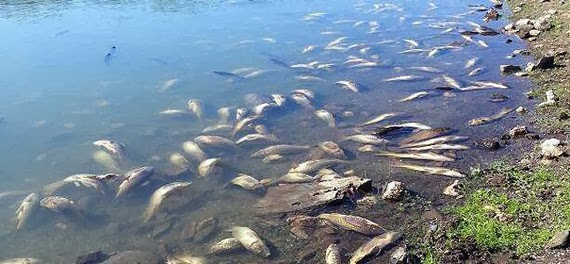
\includegraphics[width=\textwidth]{Figures/spaindeadfish.jpg}\end{figure}}
						\only<3>{\begin{figure}\centering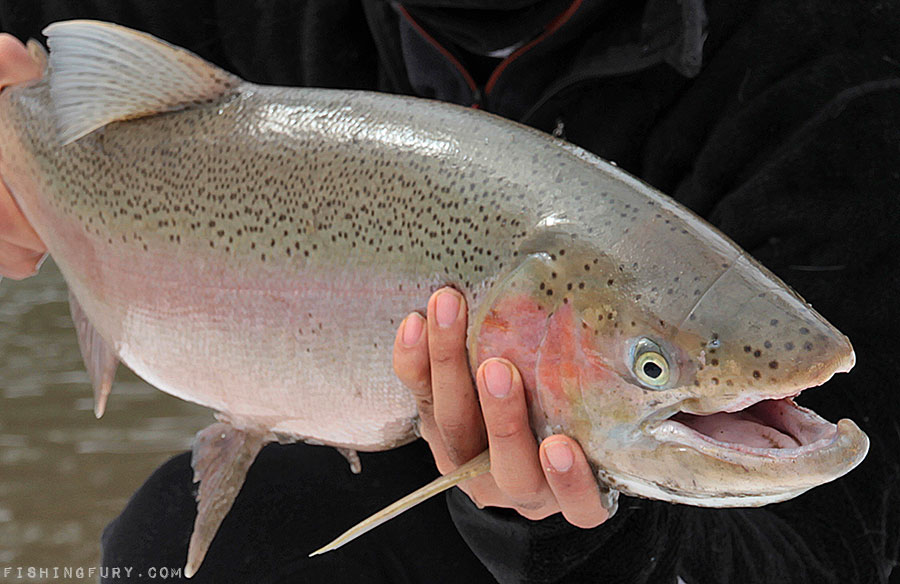
\includegraphics[width=.88\textwidth]{Figures/happy-trout1.jpg}\end{figure}}			
			\end{columns}
\end{frame}